\chapter{3D Reconstruction Method}

\section{Preprocessing}
	The images used have already been stereo rectified. We use the grabcut algorithm, 
which is based on graph cuts, to extract the foreground and mask the surrounding background.

\begin{figure}[H]
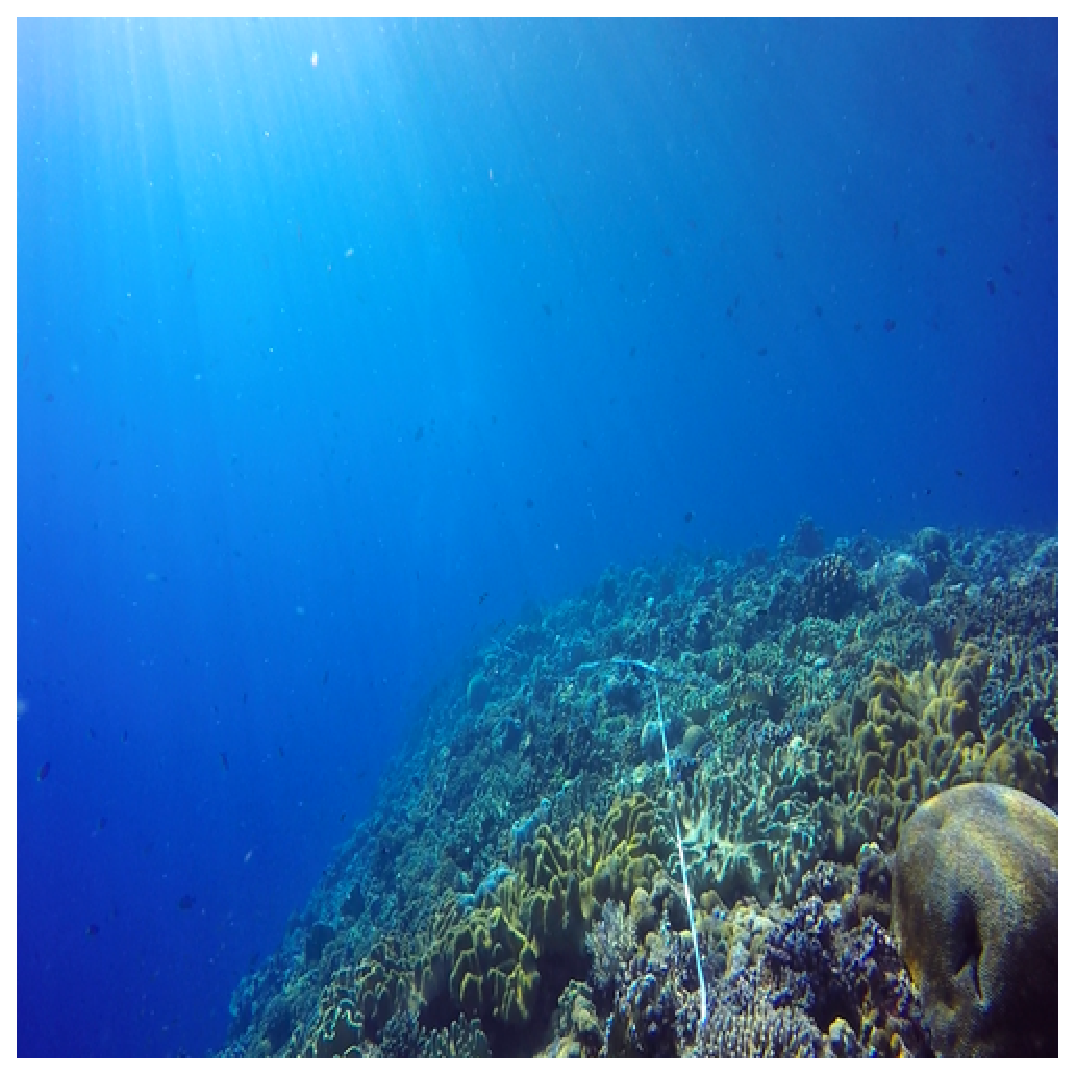
\includegraphics[width=0.8\textwidth, height=0.4\textwidth]{unmasked.eps}
\caption{Raw Rectified Image}
\end{figure}

\begin{figure}[H]
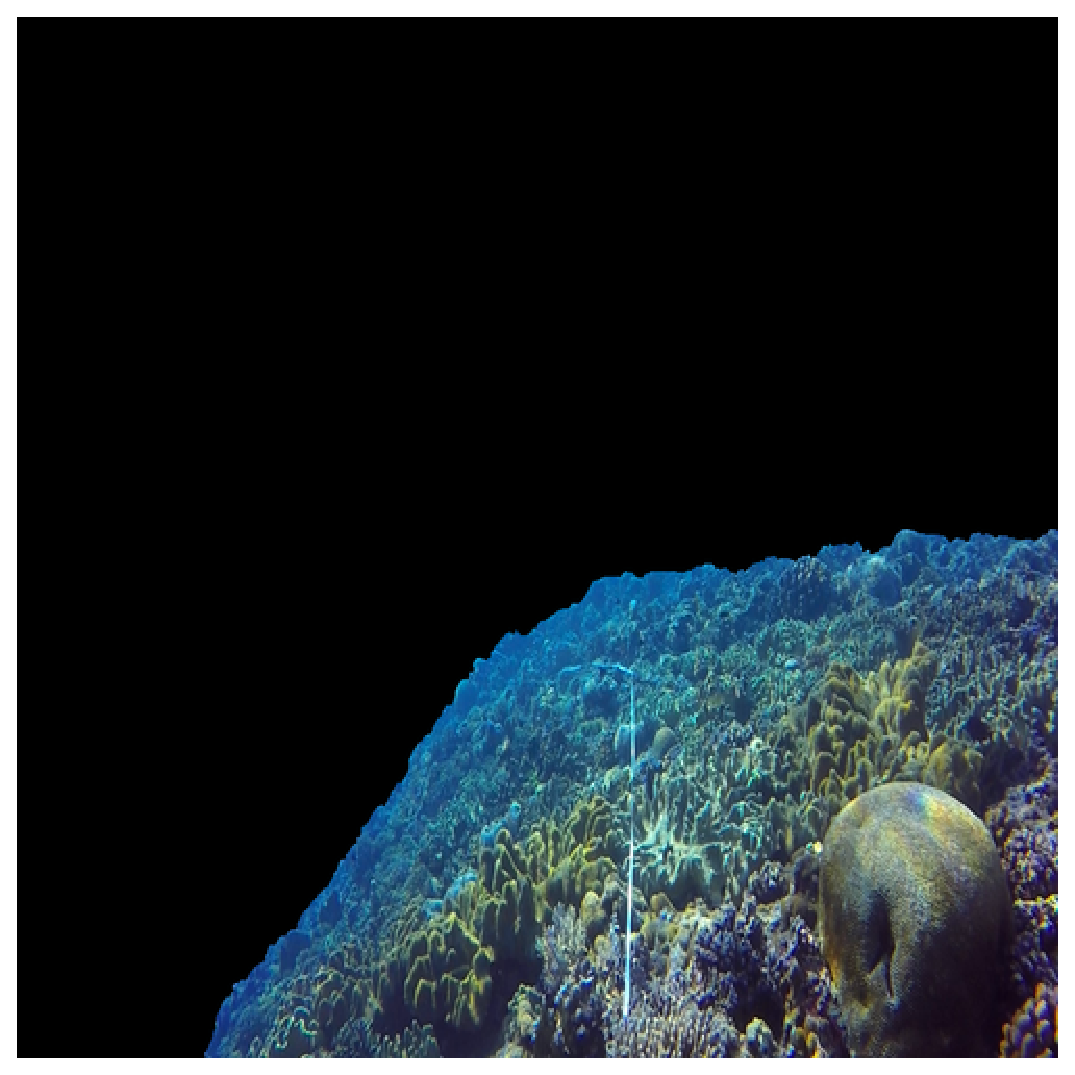
\includegraphics[width=0.8\textwidth, height=0.4\textwidth]{masked-1.eps}
\caption{Masked Rectified Image}
\end{figure}




\section{Generating the Disparity Map}

	The stereo matching algorithm used was based on Hirschmuller's, Semiglobal Matching stereo
method \cite{sgm}. It's called Semi Global Block Matching algorithm(SGBM). I tweaked the parameters for best results. After generating the disparity map, I used a weighted least squares filter to smoothen the initial dense disparity map. Next, we compute the the point cloud based from the dense disparity map.

\begin{figure}[H]
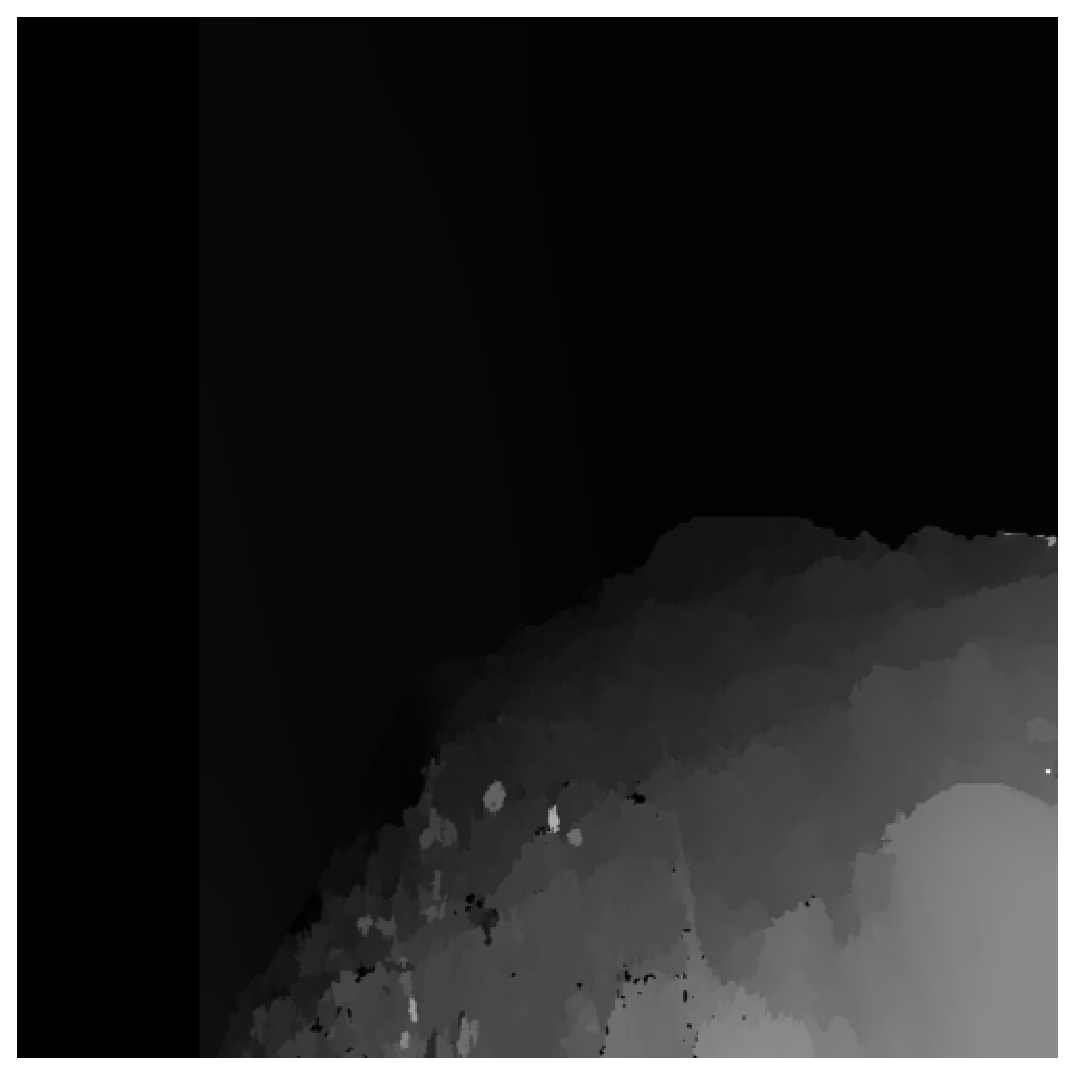
\includegraphics[width=0.8\textwidth, height=0.4\textwidth]{disp_map.eps}
\caption{Generated disparity map}
\end{figure}



\section{Interframe Reconstruction}
*not yet done*

\section{Meshing of Point Cloud}

I'm currently using Meshlab to create a mesh. The generated point cloud consists of 300,000+ points. In my meshing, I initially use poisson sampling to reduce the points and apply the ball-pivoting algorithm for surface reconstruction by Bernardini et. al.
    
